% Drawing 154/03-10 -- folder 154, batch 03, archive page 59 (PDF page 60).
% Transcription: figure au bas de la colonne : deux droites orange verticales et une droite orange horizontale $D_0$ ; une droite verte $D$, parallèle à $D_0$ au-dessus d'elle, s'infléchit pour la rejoindre et la croiser près du point $s$ ; le point $a$ est marqué sur $D$, et la région entre $D$ et $D_0$ près de $s$ est hachurée au crayon
% Kind: line D crossing D_0 near s. Method 2 (schematic redraw from the facsimile). Status: ok.
% Notes: Foot of the right column: two vertical orange lines and a horizontal orange line D_0; the green line D, parallel to D_0 and above it on the right, bends down to meet it and cross it near the point s (on the left vertical), and runs below D_0 to the left; the point a is marked on D (a black point where D meets the right vertical); the region between D and D_0 near s is hatched in pencil.
% Coordinates: 1 unit = 1 mm = 1/100 of the crop width (bbox in page fractions: [0.624, 0.444, 0.937, 0.521]).
% Redrawn by Claude (claude-opus-5-5), issue #73, 2026-11-07; not checked by a human; not compiled (no TeX in the session).
% Rights: reproduces part of the work -- behind RENDER_TRANSCRIPTS, never published by itself.
\documentclass[tikz,border=3pt]{standalone}
\usepackage{amsmath,amssymb}
\usetikzlibrary{patterns,arrows.meta}
\tikzset{Or/.style={orange!90!black}, Ye/.style={yellow!80!orange}, Lg/.style={green!60!black!70}, Dg/.style={green!45!black}, Br/.style={brown!80!black}, Rd/.style={red!85!black}, Bl/.style={blue!70!black}, Gy/.style={black!40}, pencil/.style={black!45}, struck/.style={black!35}, mark/.style={circle,draw,inner sep=1.3pt}, pt/.style={circle,fill,inner sep=0.9pt}, opt/.style={circle,draw,fill=white,inner sep=1.1pt}}
\begin{document}
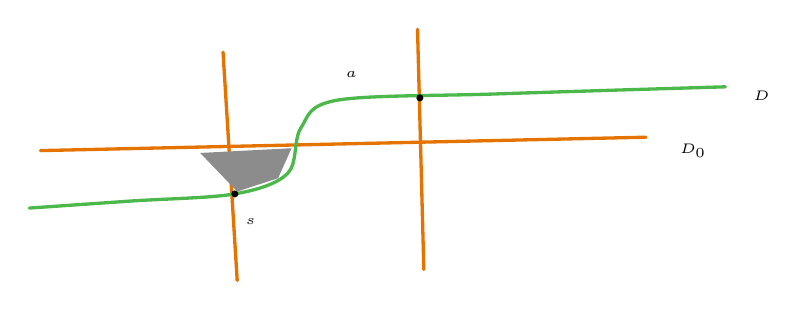
\begin{tikzpicture}[x=1mm,y=1mm,line cap=round,line join=round,font=\scriptsize]
\draw[Or,very thick] (27.5,-4.3) -- (29.3,-33.3);
\draw[Or,very thick] (52.2,-1.4) -- (53,-31.9);
\draw[Or,very thick] (4.3,-16.8) -- (81.2,-15.1);
\node[inner sep=1pt] at (87.2,-16.8) {\tiny $D_0$};
\draw[Lg,very thick] plot[smooth, tension=0.55] coordinates {(2.9,-24.1) (15.9,-23.2) (29,-22.3) (35.7,-19.7) (37.4,-13.9) (42,-10.4) (62.3,-9.6) (91.3,-8.7)};
\node[inner sep=1pt] at (95.9,-9.9) {\tiny $D$};
\node[pt] at (29,-22.3) {};
\node[inner sep=1pt] at (31,-25.8) {\tiny $s$};
\node[pt] at (52.5,-10.1) {};
\node[inner sep=1pt] at (43.8,-7.2) {\tiny $a$};
\fill[pattern=north east lines,pencil] (24.6,-17.1) -- (36.2,-16.5) -- (34.5,-20.3) -- (29.3,-22) -- cycle;
\end{tikzpicture}
\end{document}
